\section{Design Decisions and Challenges}
\label{sec:background}

In Presto, we make several design choices to 
build a highly robust and scalable system that provides near optimal load 
balancing without requiring changes to the transport layer or switch hardware. We 
now discuss our design decisions.


\subsection{Design Decisions}

\tightparagraph{Load Balancing in the Soft Edge} A key design decision in Presto 
is to implement the functionality in the soft edge (\ie{}the vSwitch and hypervisor) of 
the network. 
%should we motivate why not to do it in hardware?
%A current trend in datacenter design is to utilize network equipment from 
%original design manufacturers (ODMs) in order to simplify and customize
%the network. This has been reported to significantly reduce costs and improve
%network performance~\cite{aws-peek}.
%Motivation here is that network is becoming very simple, and functionalities
%are being moved to an intelligent edge. Examples are VMWare/NSDI, Fabric, NFV in vSwitch,
%SDNs/OpenFlow, 
% Given recent advancements in this space\eric{what advancements? can we be more specific
% in order to provide better motivation?}, we believe the soft edge is the best 
% place to deploy new network functions, such as load balancing, in a scalable and 
% distributed manner.\eric{is this a new position? vmware nsdi paper...}
The vSwitch occupies a unique position in the networking stack 
in that it can easily modify packets without requiring any changes to customer VMs or transport layers.
Functionality built into the vSwitch can be made aware of the underlying hardware offload
features presented by the NIC and OS, meaning it can be fast.
Furthermore, an open, software-based approach prevents extra hardware cost and vendor 
lock-in, and allows for simplified network management. 
These criteria are important for providers today~\cite{aws-peek}.
Thanks to projects like Open vSwitch, 
soft-switching platforms are now fast, mature, open source, adopted widely, remotely 
configurable, SDN-enabled, and feature-rich~\cite{ovs-edge,nv-mtd,pfaff2015design}. Presto is built on these 
platforms.

\tightparagraph{Reactive vs Proactive Load Balancing} The second major design decision in 
Presto is to use a proactive approach to congestion management. Bursty 
behavior can create transient congestion that must be reacted to 
before switch buffers overflow to prevent loss (timescales range from 100s of $\mu$s 
to around 4 ms~\cite{planck}). This requirement renders most of the centralized reactive schemes ineffective
as they are often too slow to react to any but the largest network events,~\eg{}link failures. 
%Not reacting to transient congestion can increase tail latencies.
Furthermore, centralized schemes can hurt performance when rerouting
flows using stale information.
%By reacting on a different scale than the congestion, centralized schemes may reroute flows
%on stale information, which can hurt performance.
Distributed reactive schemes like MPTCP~\cite{mptcp} and 
CONGA~\cite{conga} can respond to congestion at faster timescales, but have a high barrier to deployment.
Furthermore, distributed reactive schemes must take great care to avoid oscillations.
Presto takes a proactive, correct-by-design approach to congestion management. 
That is, if small, near-uniform portions of traffic are equally
balanced over a symmetric network topology, then the load-balancing can remain agnostic to congestion and
leave congestion control to the higher layers of the networking stack.
%then we don't need to 
%be reactive to congestion.
Presto is only reactive to network events such as link failures. Fortunately, 
the larger timescales of reactive feedback loops are sufficient in these scenarios. 

\tightparagraph{Load Balancing Granularity} ECMP has been shown to be ineffective at load balancing the network, and thus many schemes advocate load balancing at a finer granularity than a flow~\cite{drb,conga,juniper-vcf,packetspray}. A key factor impacting the choice of granularity is operating at high speed. 
%and ensuring suitable application level performance.
%Implementing fine-grained, near-uniform load balancing in 10+ Gbps networks
%is difficult.
Operating at 10+ Gbps incurs great computational overhead, and therefore host-based load balancing schemes
must be fast, light-weight and take advantage of optimizations provided in the networking stack.
For example, per-packet load balancing techniques~\cite{drb} cannot be
employed at the network edge because TSO does not work on a per-packet
basis. TSO, commonly supported in OSes and NICs, allows for large TCP segments (typically 64 KB in size)
to be passed down the networking stack to the NIC. The NIC breaks the segments into MTU-sized packets and copies and computes
header data, such as sequence numbers and checksums. When TSO is disabled, a host incurs 100\% utilization of one CPU core and can only achieve
around 5.5 Gbps~\cite{bullettrains}. Therefore, per-packet schemes are unlikely to scale to fast networks without hardware support.
Limiting overhead by increasing the MTU is difficult because
VMs, switches, and routers must all be configured appropriately, and traffic
leaving the datacenter must use normal 1500 byte packets. Furthermore, per-packet schemes~\cite{drb,packetspray} are likely to
introduce significant reordering into the network.
%Achieving line rate at 10 Gbps is nontrivial because dealing
%with so many 1500 byte MTU-sized packets at varying layers
%of the networking stack causes significant computational overhead.
%Therefore, modern operating systems and network adapters have many
%optimizations to help burden the load.
%On the sender side, TCP Segmentation Offload (TSO)~\footnote{Generically known as large segment offload or generic segmentation offload}
%is designed to allow the TCP/IP stack to deal with large TCP segments. Segments, up to 64 KB in size, are passed
%from the application layer all the way down to the NIC, which in turn breaks the large segment down into 1500 byte packets.
%The NIC copies and calculates the header information, such as checksums and sequence numbers.
%This allows the computational burden to be substainally lessened, and therefore rates of 10+
%Gbps can be achieved. With TSO disabled, achievable 10 Gbps throughput drops to around 5.5 Gbps~\cite{bullettrains}.



\begin{figure}[!t]
        \centering
  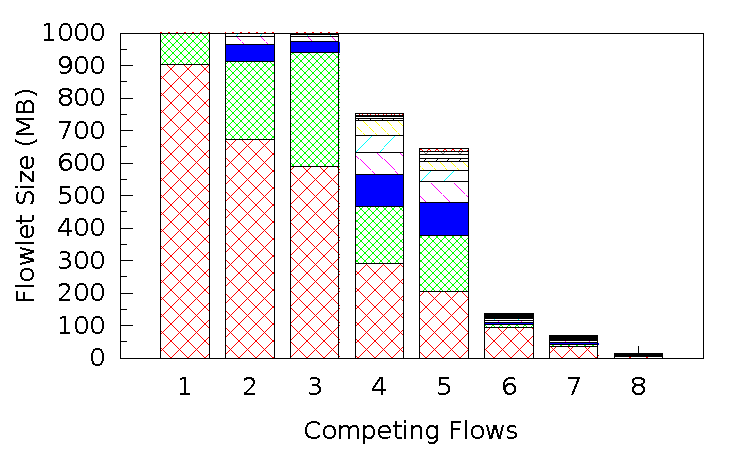
\includegraphics[width=0.7\textwidth]{presto/figures/flowlets/histo.pdf}
        \caption{Stacked histogram of flowlet sizes (in MB) for a 1 GB {\tt scp} file transfer. We vary the number of {\tt nuttcp}~\cite{nuttcp} background flows and
                denote them as {\em Competing Flows}. The size of each flowlet is shown within each bar, and flowlets
                are created whenever there is a 500 $\mu$s delay between segments. The top 10 flowlet sizes are shown here.
                We also analyzed the results of a 1 GB {\tt nuttcp}, {\tt ftp}, and a simple custom client/server transfer and found them
                to be similar. }
        \label{micro_flowlet_size}
\end{figure}

%\aditya{the following two paras don't flow well. they don't make a clear case for why flowlets is a bad idea and TSO segment level switching is a good idea. if reordering is the 100us flowlets' big problem then why not use our receiver-side reordering tricks with 100us flowlets? also it is not clear how were are overcoming reordering simply by relying on TSO segment switching}

%\eric{Rough estimates from our experiments with 100$\mu$s: ~90\% of flowlet sizes are 114KB or less with flowlets. ~00.1\% of flowlets are
%larger than 1 MB, with the largest ranging from 2.1-20.5MB. Some thoughts: (i) 100 $\mu$s flowlets can still have flowlet sizes larger 
%than switch buffers, which can cause congestion/loss when collision occur, (ii) given that flowlet with 100 $\mu$s does not prevent reordering,
%then why should we use flowlets at all? (iii) flowlets were really meant to have inactivity timers larger than the max difference in latency
%over any two paths, and buffer latency at one switch alone is ~4ms, so the use of flowlets on these small time scales is fundamentally
%flawed, (iv) flowlets are sensitive to traffic demand at sender, (v) flowlets are non-uniform in size, (vi) flowlets could break small 
%flows over multiple paths. Using TSO segment ensures: (i) small, uniform units of load-balancing, which means (ii) we are indenpendent
%of traffic demand, (iii) collisions are not a problem b/c TSO size is smaller than buffer size, (iv) most small flows are routed
%over the same path, (v) we do not impose too much computational overhead on sender/receiver and (vi) we still need to solve reordering.}

% Rough outline for next two paragraphs
% Problem with flowlets:
%  1. Sensitive to traffic patterns at the sender
%     a. In practice, we find this means the distribution of flowlet sizes is not uniform, and has a tail
%     b. These tails can still experience hash collisions, albeit less often.
%		i. congestion: lower throughput and to longer mice tail latencies
%  2. Needlessly break down small flows into several flowlets
%     a. Especially early in connection: 100us, 50 KB mice flows broken into 4-5 flowlets
%  3. Designed to be robust to reordering, but difficult to tune
%


Another possibility is to load balance on flowlets~\cite{conga,juniper-vcf}.  
A flow is comprised of a series of bursts, and a flowlet is created when
the inter-arrival time between two packets in a flow exceeds a threshold inactivity timer.  
In practice, inactivity timer values are between 100-500 $\mu$s~\cite{conga}. 
These values intend to strike a good balance between load balancing on a sub-flow level 
and acting as a buffer to limit reordering between flowlets.
Flowlets are derived from traffic patterns at the sender, and in practice this
means the distribution of flowlet sizes is not uniform. To analyze flowlet sizes, a simple experiment is shown in Figure~\ref{micro_flowlet_size}. 
We connect a sender and a receiver to a single switch and start an {\tt scp} transfer designed to 
emulate an elephant flow. Meanwhile, other senders are hooked up to the same switch and
send to the same receiver. We vary the number of these competing flows and show a stacked histogram of 
the top 10 flowlet sizes for a 1 GB {\tt scp} transfer with a 500 $\mu$s inactivity timer. 
The graph shows flowlet sizes can be quite large, with more than half the transfer being attributed
to a single flowlet for up to 3 competing flows. Using a smaller inactivity timer, such 100$\mu$s, helps (90\% of flowlet sizes are 114KB or less), but
does not prevent a long tail: 0.1\% of flowlets are larger than 1 MB, with the largest ranging from 2.1-20.5 MB.
Collisions on large flowlet sizes can lead to congestion.
The second problem with flowlets is that small inactivity thresholds, such as 100 $\mu$s, can lead to significant reordering.
Not only does this impact TCP performance (profiled in Section~\ref{sec:micro}), but it also needlessly 
breaks small flows into several flowlets. With only one flow in the network, we found a 50 KB
mice flow was broken into 4-5 flowlets on average. Small flows typically do not need to be
load balanced on a sub-flow level and need not be exposed to reordering.


%Another possibility is to load balance on flowlets~\cite{conga,juniper-vcf}.  A flow is typically comprised of a series of bursts, and each burst is defined as a flowlet. By monitoring the inter-arrival time of packets in a flow, one can easily define an inactivity timer to seperate flowlets.  In practice, intactivity timer values are between 100-500 $\mu$s~\cite{conga}. These values are intended to strike a good balance between creating enough opportunities to load balance on a sub-flow level and also ensure the reordering is limited at the destination due to the time buffer naturally incurred between flowlets.  We find, however, that it is difficult to strike a balance between achieving fine-grained, near-optimal load balancing and robustness against reordering. We perform a simple experiment in Figure~\ref{micro_flowlet_size}.  We connect a sender and a receiver to a single switch and start a transfer over an application designed to emulate an elephant flow ({\tt scp}). Meanwhile, we also hook up other senders to the same switch and have them send to the same reciever. We vary the number of competing flows and show a stacked histogram of the top 10 flowlet sizes for a 1 GB scp transfer with a 500 $\mu$s inactivity timer. \eric{Competing flows use nuttcp.} The graph shows flowlet sizes can be large, which means hash collisions can still occur on large flowlets.  Using a smaller timeout, such as 100 $\mu$s, creates smaller flowlets, but as we show in Section XXX, suffers from severe reordering that greatly reduces throughput and hurts applications.  \eric{mention creates congestion, which leads to lower thorughput and increase mice FCT latency}

% What do we want in sub-flow load balancing?
%  A. Want to move toward idealized ECMP: uniform sub-flow load balancing without the tail
%  B. Units should be as small as possible for fine-grained load balancing, but
%       not so small to be inefficient (TSO) or break small flows into parts
%  C. Independent of traffic patterns on sender
%  As a result, we settle on...

The shortcomings of the previous approaches lead us to reconsider on what granularity
load balancing should occur. 
%We take motivation from a best-case ECMP scenario. 
Ideally, sub-flow load balancing should be done on near uniform sizes.
%independent of traffic patterns on the sender to avoid long tails. 
Also, the unit of load balancing should be small to
allow for fine-grained load balancing, but not so small as to break small flows into 
many pieces or as to be a significant computational burden. As a result, we
propose load balancing on 64 KB units of data we call {\em flowcells}. Flowcells
have a number of advantages. First, the maximum segment size supported by TSO
is 64 KB, so flowcells provide a natural interface to high speed optimizations provided
by the NIC and OS and can scale to fast networking speeds. Second, an overwhelming fraction of mice flows are less than 64 KB in size
 and thus do not have to worry about reordering~\cite{benson10,vl2,kandula2009nature}.
Last, since most bytes in datacenter networks originate from elephant flows~\cite{kandula2009nature,benson10,dctcp},
this ensures that a significant portion of datacenter traffic is routed on uniform
sizes. While promising, this approach must combat reordering to be effective. 
Essentially we make a trade-off: 
%we provide line rate load balancing in the most effective
%manner as to avoid congestion and then handle reordering head-on at the receiver.
the sender avoids congestion by providing fine-grained, near-uniform load balancing,
and the receiver handles reordering to maintain line-rate.


%We highlight the challenges of this approach
%in the next subsection and provide a design to mitigate reordering problems in Section~\ref{sec:design}.

%In order to obtain fine-grained, near-optimal load balancing, we should stripe on a granularity
%that is indendpent of traffic patterns, near-uniform in size, and as small as possible while still
%scaling to fast network speeds.
%Therefore, we argue the TSO segment~\keqiang{what about saying maximum TSO segment size (64KB), each TSO segment's size is bounded by maximum TSO size} 
%is the natural granularity in which to load balance. Doing so
%provides several benefits. First, TSO segments are small and near-uniform in size, so an
%effective load-balancing scheme should be able to closely track the optimal case of per-packet
%load balancing, but without the additional computational overhead.
%Second, the TSO engine in the NIC will ensure that all packets created from a TSO segment will contain the same
%header information. We show in Section XXX how this is important to deal with reordering because
%we can easily impart metadata on all packets within a segment that help us distinguish loss from 
%ordering~\keqiang{all the packets within the same flowcell contain the same flowcell id.  
%"all packets created from a TSO segment will contain the same
%header information" is fine but a flowcell can contrain several TSO segments depending on TSO segment size}.
%Last, small flows less than 64 KB in size will actually be routed over the
%same path in the network, meaning a very large fraction of mice flows will not be routed on a subflow
%level and thus do not have to worry about reordering~\cite{benson10,vl2,kandula2009nature}~\keqiang{Around 90\% of datacenter flows' sizes are smaller than 64KB~\cite{benson10}, 
%meaning the overwhelming majority is load balanced like ECMP and we only need to engineering the left 10\%}.
%\eric{need to mention that we can combine segments as long as not above 64 KB, so not really
%per TSO segment. helps in small flows.}
%While promising, this approach has a major challenge: reordering. We highlight these challenges
%in the next subsection and provide a design to mitigate the problems in Section~\ref{sec:design}.

\tightparagraph{Per-Hop vs End-to-End Multipathing}
The last design consideration is whether multipathing should be done on a local, per-hop level (\eg{}ECMP), or
on a global, end-to-end level. In Presto, we choose the latter: pre-configured end-to-end paths
are allocated in the network and path selection (and thus multipathing) is realized by having the network edge
place flowcells onto these paths. 
Presto can be used to load-balance in an ECMP style per-hop manner, but the choice of end-to-end 
multipathing provides additional benefits due to greater control of how flowcells are mapped to
paths. Per-hop multipathing can be inefficient
under asymmetric topologies~\cite{wcmp}, and load-balancing on a global end-to-end level can allow
for weighted scheduling at the vSwitch to rebalance traffic. This is especially important when failure occurs.
The second benefit is flowcells can be assigned over multiple paths very evenly
by iterating over paths in a round-robin, rather than randomized, fashion. 

%As we show
%in Section~\ref{sec:micro}, randomization in per-hop multipathing can lead to "unluckiness" where
%multiple flowcells get sent to the same link over a small timescale by multiple flows. This transient congestion
%can lead to increased buffer occupancy and higher delays in the network. These benefits can
%fundamentally be provided at the per-hop level (\cite{wcmp} handles asymmetry), but require changes to networking firmware. 
%These considerations motivate us to utilize end-to-end multipathing, but Presto can also
%use per-hop multipathing when conveinent.

\subsection{Reordering Challenges}
%The above design decisions in Presto cause following main challenges:
Due to the impact of fine-grained, flowcell-based load balancing, Presto must account for reordering. Here, we 
highlight reordering challenges. The next section shows how Presto deals with these concerns.

%\tightparagraph{Soft Edge Distributed Load Balancing}
%There are two main challenges in implementing load balancing at the soft edge. First, the implementation
%must scale to fast networking speeds because networking at 10+ Gbps can have significant overhead if not carefully
%considered. Therefore, in order to achieve line rate, great care must be taken to ensure that load balancing
%schemes are light-weight, simple and can take advantage of optimizations provided by the NIC and OS.  
%The second major problem is how to load balance in a distributed fashion at the vSwitches in such
%a way that the load balancing performs well globally.
%Nodes must ensure they are spreading
%their traffic equally throughout the network, but in a low-overhead fashion that does not require detailed
%topographical information about the network, real-time traffic matrices, or strict coordination
%with other senders.

%\eric{several things to add: in presto, we can just make dumb edge decisions and not have to worry
%about (i) the traffic patterns, that is who else is sending, (ii) topology asymmetry. Basically,
%we want to highight that the vSwitch shouldn't require a lot of detailed network-wide information,
%but should be able to somehow still load balance in a way that performs very well globally.}

\tightparagraph{Reordering's Impact on TCP} The impact of reordering on TCP is well-studied~\cite{leung2007overview,paxson1997end}. 
Duplicate acknowledgments caused by reordering
can cause TCP to move to a more conservative sender state and reduce the sender's congestion window.
Relying on parameter tuning, such as adjusting the DUP-ACK threshold, is not ideal because 
increasing the DUP-ACK threshold increases the time to recover from real loss. Other TCP settings
such as Forward Acknowledgement (FACK) assume un-acked bytes in the SACK are lost and degrade
performance under reordering. 
A scheme that introduces reordering should not rely on careful configuration of TCP parameters
because (i) it is hard to find a single set of parameters that work effectively over multiple 
scenarios and (ii) datacenter tenants should not be forced to constantly tune their networking stacks.
Finally, many reordering-robust variants of TCP have been proposed~\cite{rr-tcp,blanton2002making,tcp-pr}, but
as we will show, GRO becomes ineffective under reordering. Therefore, reordering should
be handled below the transport layer.

\tightparagraph{Computational Bottleneck of Reordering}
Akin to TSO, Generic Receive Offload (GRO) mitigates the computational burden of receiving
1500 byte packets at 10 Gbps. GRO is implemented in the kernel of the hypervisor,
and its handler is called directly by the NIC driver. It is responsible
for aggregating packets into larger segments that are pushed up to OVS and the TCP/IP stack. 
GRO is implemented in the Linux kernel and is used even without virtualization. Similar
functionality can be found in Windows (RSC~\cite{ms-rsc}) and hardware (LRO~\cite{grossman2005large}).

Because modern CPUs use aggressive prefetching, the cost of receiving
TCP data is now dominated by per-packet, rather than per-byte, operations.
As shown by Menon~\cite{optimize-tcp-receive},  the majority of this overhead comes from
buffer management and other routines not related to protocol processing, and therefore 
significant computational overhead can be avoided by aggregating "raw" packets from
the NIC into a single {\tt sk\_buff}.
%\footnote{Refer to~\cite{linuxgro,optimize-tcp-receive} for detailed study and explanation}
Essentially, spending a few cycles to aggregate packets within GRO creates less segments for
TCP and prevents having to use substantially more cycles at higher layers in the networking stack.
Refer to~\cite{linuxgro,optimize-tcp-receive} for detailed study and explanation.

To better understand the problems reordering causes, a brief description of  
the TCP receive chain in Linux follows. First, interrupt coalescing allows the NIC to create an interrupt for a batch of packets~\cite{mogul1997eliminating,understanding-linux-network},
which prompts the driver to poll the packets into an aggregation queue. Next, the driver
invokes the GRO handler, located in the kernel, which
{\em merges} the packets into larger segments. The merging continues,
possibly across many polling events, until a segment
reaches a threshold size, a certain age, or cannot be combined with the incoming packet. Then, the
combined, larger segment is {\em pushed up} to the rest of the TCP/IP networking stack. The GRO process is
done on a per-flow level. With GRO disabled, throughput drops to around
5.7-7.1 Gbps and CPU utilization spikes to 100\% (Section~\ref{sec:micro} and~\cite{bullettrains}). 
Receive offload algorithms, whether in hardware (LRO)~\cite{grossman2005large,open-lro} or in software (GRO), are usually
{\em stateless} to make them fast: no state is kept beyond the segment being merged.


%\begin{figure}[!htb]
%        \centering
%  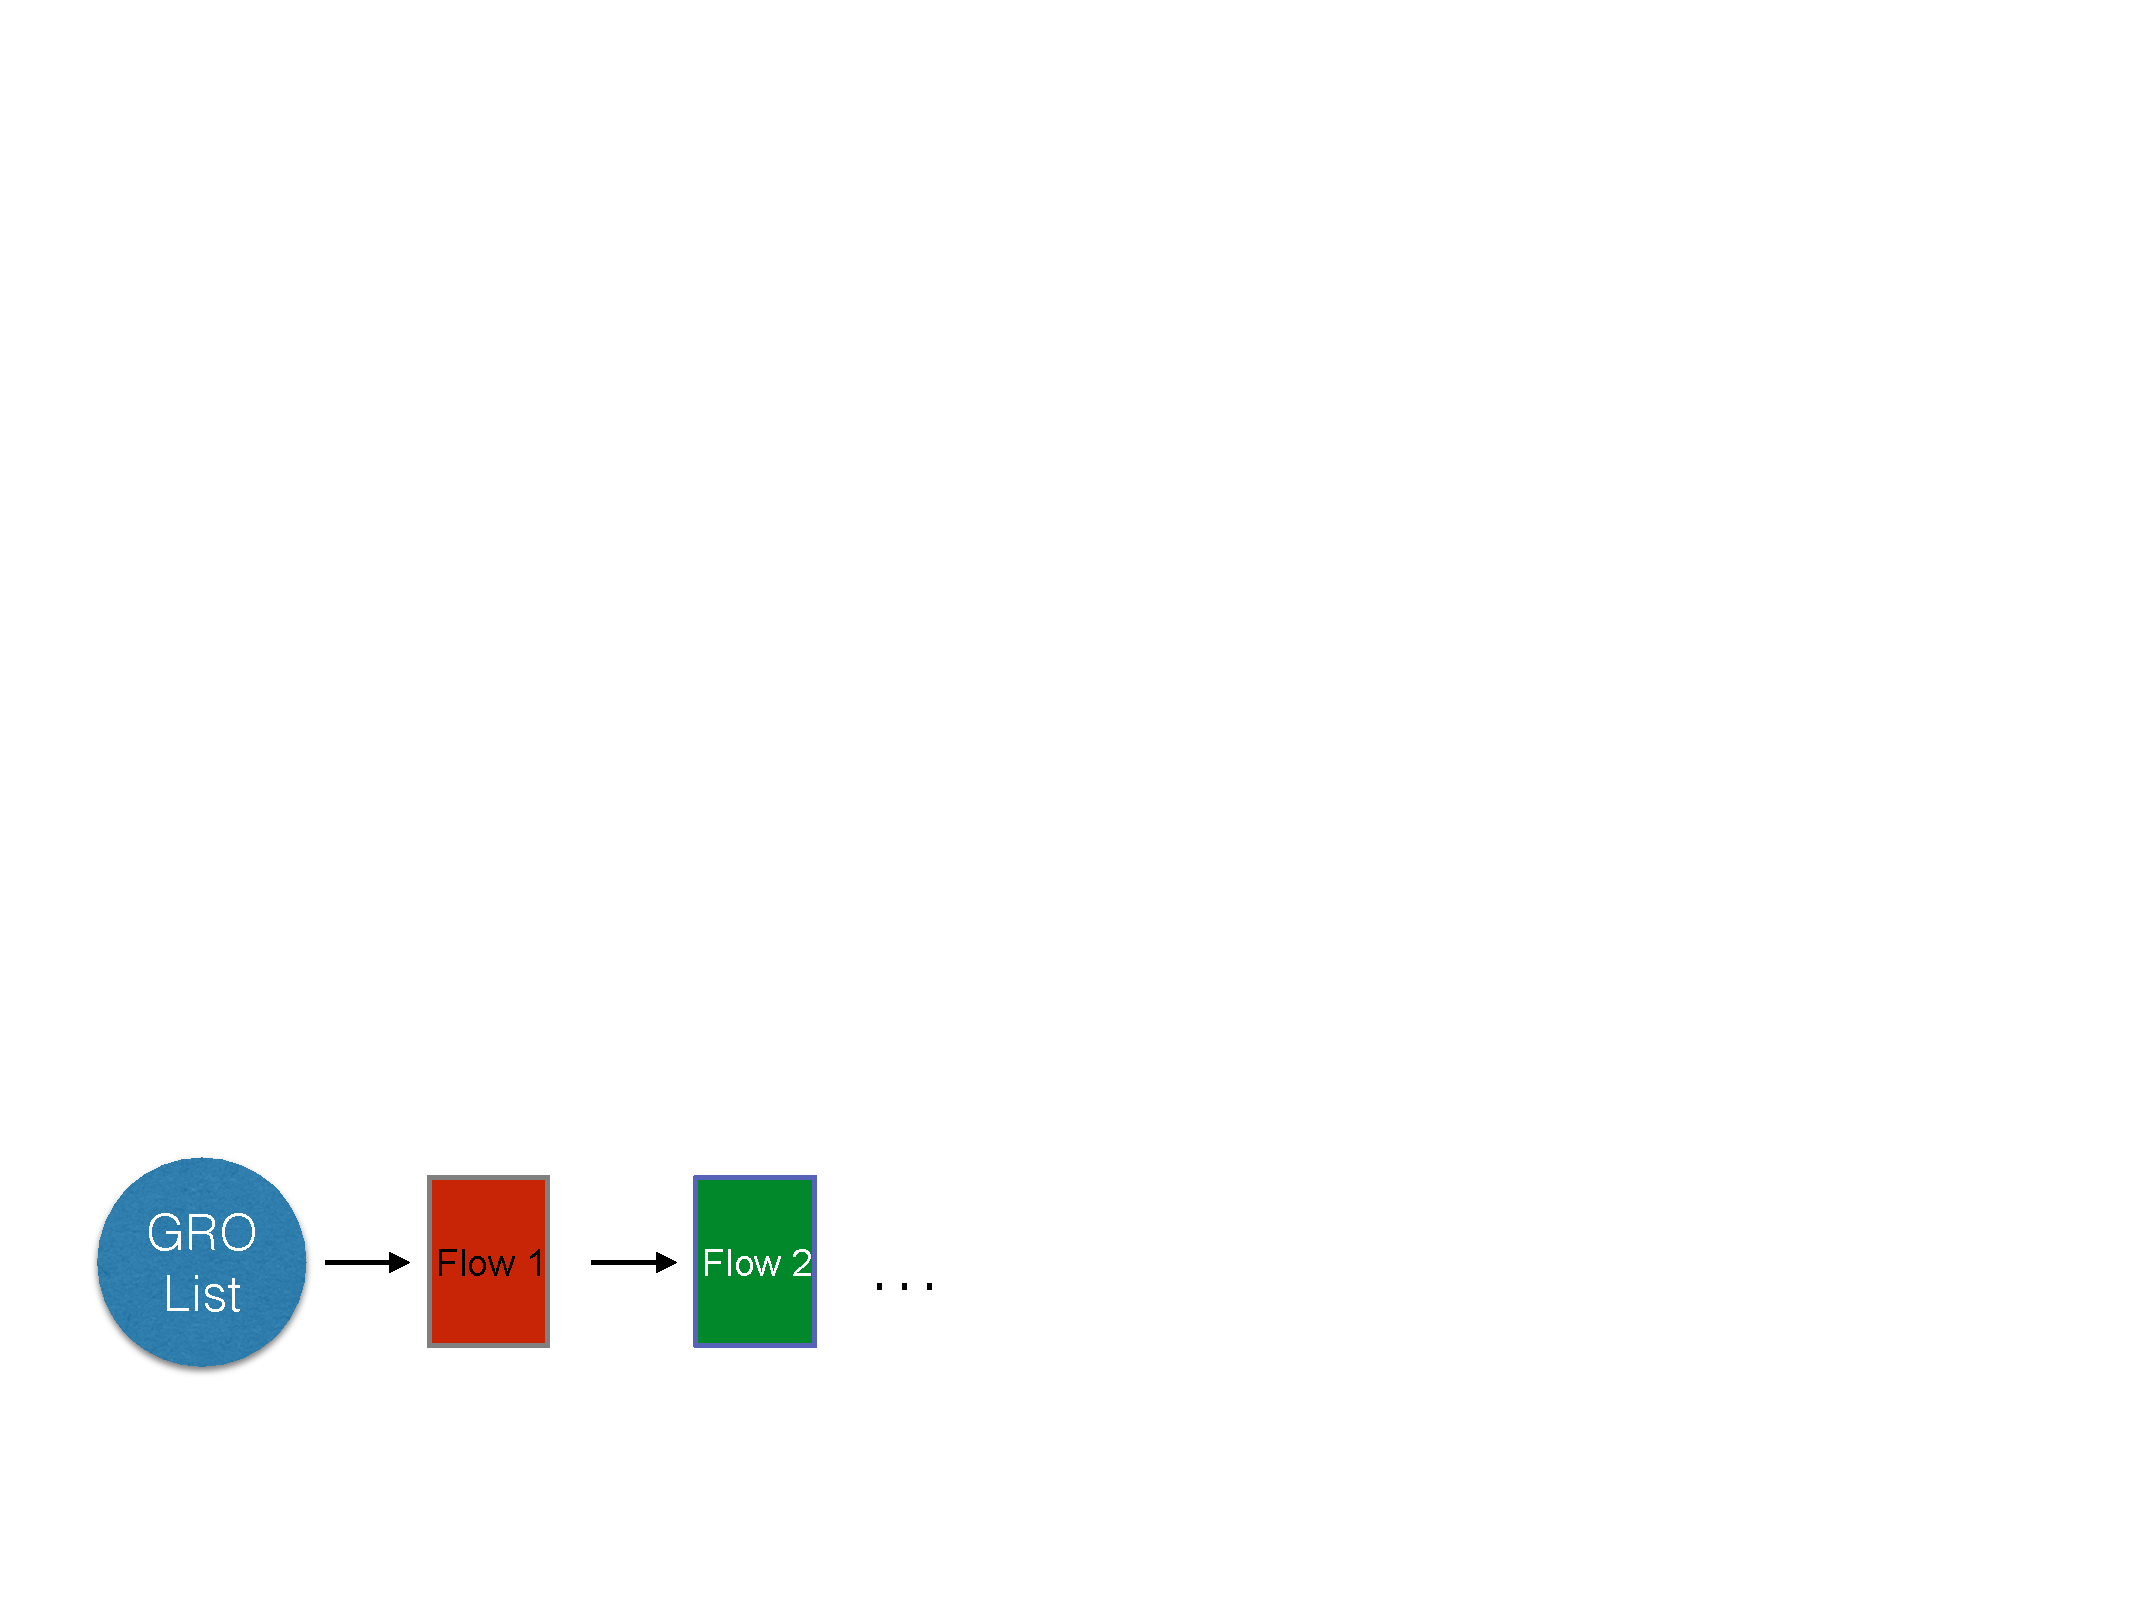
\includegraphics[width=0.45\textwidth]{presto/figures/gro-design/gro.pdf}
%        \caption{GRO design. FIX ME!}
%        \label{gro-design}
%\end{figure}

\begin{figure}[!t]
        \centering
  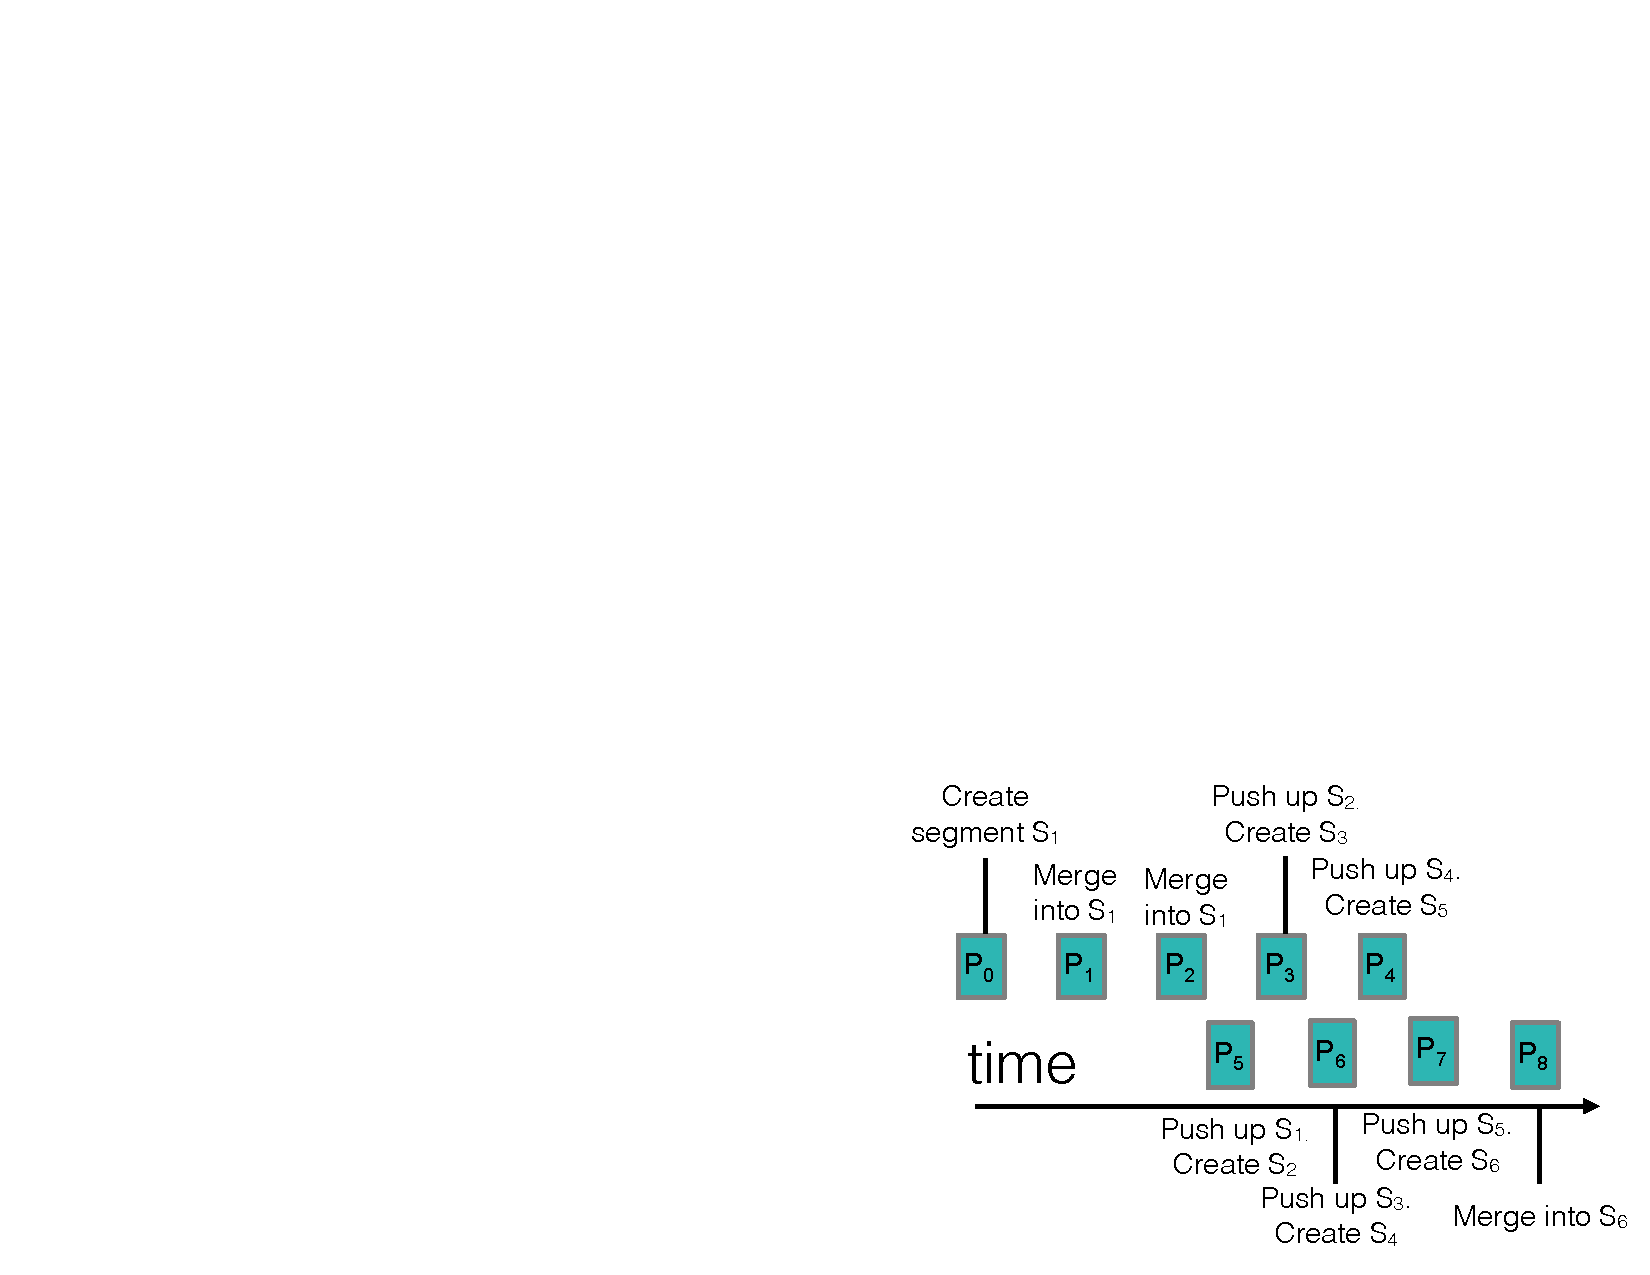
\includegraphics[width=0.7\textwidth]{presto/figures/gro-design/gro-break.pdf}
        \caption{GRO pushes up small segments ($S_i$) during reordering.}
        \label{gro-break}
\end{figure}


We now uncover how GRO breaks down in the face of reordering. Figure~\ref{gro-break} shows the impact of reordering on GRO.  Reordering does not allow the segment to grow: each reordered packet cannot be merged with the existing segment, and thus the previously created segment must be pushed up. With extreme reordering, GRO is effectively disabled because small MTU-sized segments are constantly pushed up. This causes (i) severe computational overhead and (ii) TCP to be exposed to significant amounts of reordering. We term this the {\em small segment flooding} problem.

Determining where to combat the reordering problem has not previously taken the small segment flooding problem into account.  Using a reordering buffer to deal with reordered packets is a common solution (\eg{}works like~\cite{drb} re-sort out-of-order packets in a shim layer below TCP), but a buffer implemented above GRO cannot prevent small segment flooding.  Implementing a buffer below GRO means that the NIC must be changed, which is (i) expensive and cumbersome to update and (ii) unlikely to help combat reordering over multiple interrupts.

In our system, the buffer is implemented in the GRO layer itself.  We argue this is a natural location because GRO can
directly control segment sizes while simultaneously limiting the impact of reordering. 
Furthermore, GRO can still be applied on packets pushed up from LRO, which means hardware doesn't have to be modified
or made complex.
Implementing a better GRO algorithm has multiple challenges. The algorithm should be light-weight to scale to fast networking speeds. Furthermore, an ideal scheme should be able to distinguish loss from reordering.  When a gap in sequence numbers is detected (\eg{}when $P_5$ is received after $P_2$ in Figure~\ref{gro-break}), it is not obvious if this gap is caused from loss or reordering.  If the gap is due to reordering, GRO should not push segments up in order to try to wait to receive the missing gap and merge the missing packets into a preestablished segment.  If the gap is due to loss, however, then GRO should immediately push up the segments to allow TCP to react to the loss as fast as possible. Ideally, an updated GRO algorithm should ensure TCP does not perform any worse than a scheme with no reordering. Finally, the scheme should adapt to prevailing network conditions, traffic patterns and application demands.



